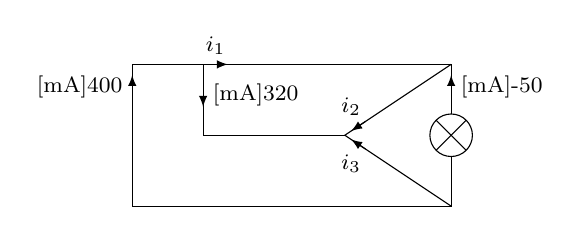
\begin{tikzpicture}[scale=.9,font=\footnotesize]
	\draw[-latex,shift={(0,.5)}](0,0)--++(0,10pt)node[midway,left]{\np[mA]{400}};
	\draw[-latex,shift={(1,1)}](0,0)--++(10pt,0)node[midway,above]{$i_1$};
	\draw[-latex,shift={(1,0.75)}](0,0)--++(0,-10pt)node[midway,right]{\np[mA]{320}};
	\draw[-latex,shift={(3,0)}](33.7:10pt)--++(213.7:7pt)node[above=2pt]{$i_2$};
	\draw[-latex,shift={(3,0)}](-33.7:10pt)--++(-213.7:7pt)node[below=2pt]{$i_3$};	
	\draw[-latex,shift={(4.5,.5)}](0,0)--++(0,10pt)node[midway,right]{\np[mA]{-50}};
	\draw (0,-1)rectangle(4.5,1);
	\draw (4.5,1)--(3,0)--(4.5,-1);
	\draw (3,0)-|(1,1);
	\pileL{}{};
	\draw[fill=white,shift={(4.5,0)}]circle(.3);
	\draw[shift={(4.5,0)}](45:.3)--(-135:.3);
	\draw[shift={(4.5,0)}](135:.3)--(-45:.3);
	% \pile{shift={(4.5,0)}}{};
	\resistanceH{shift={(3.75,.5)},rotate=33.7}{};
	\resistanceH{shift={(3.75,-.5)},rotate=-33.7}{};
	\resistanceH{shift={(2,1)}}{};
	\resistanceH{shift={(2,0)}}{};
\end{tikzpicture}
